\documentclass{beamer}

\usepackage{agda}
\usepackage{catchfilebetweentags}
\usepackage{changepage}

\usepackage{graphicx}

\graphicspath{ {./images/} }
 
\usetheme{Frankfurt}
 
%Information to be included in the title page:
\title{Qualificação}
\author{Guilherme}
\institute{FGV}
\date{2019}
 

 
\begin{document}
 
\frame{\titlepage}
 
\begin{frame}
\frametitle{Bitcoin}
\begin{itemize}
    \item É uma cripto-moeda descentralizada, sendo uma forma de dinheiro eletrônico.
    \item É considerada a primeira moeda digital mundial descentralizada, constituindo um sistema econômico alternativo (peer-to-peer electronic cash system), e responsável pelo ressurgimento do sistema bancário livre.
    \item O Bitcoin permite transações financeiras sem intermediários, mas verificadas por todos usuários (nodos) da rede, que são gravadas em um banco de dados distribuídos, chamado de blockchain, uma rede descentralizada.
\end{itemize}
\end{frame}

\begin{frame}
\frametitle{Blockchain}
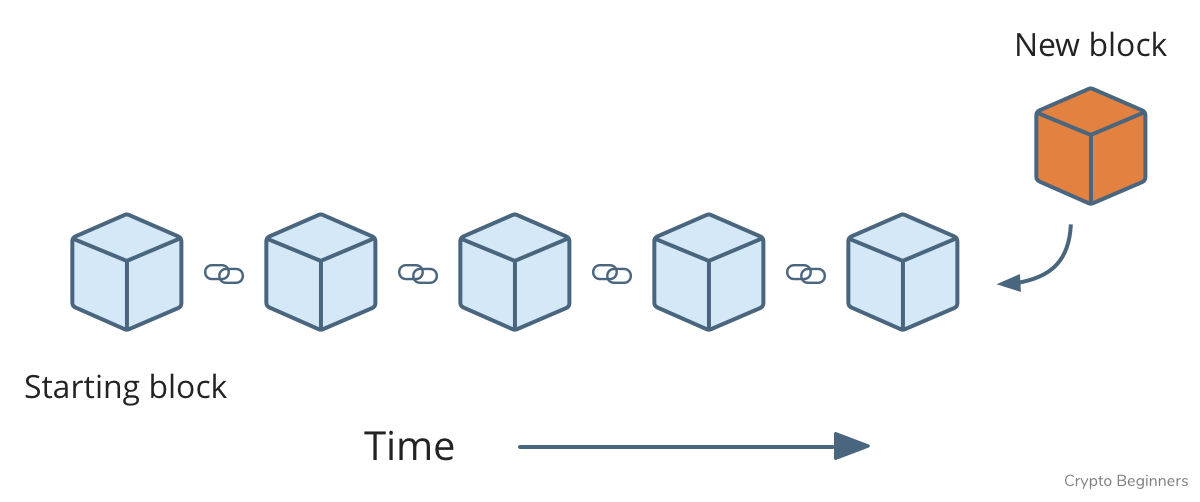
\includegraphics[width=11cm, height=8cm]{blockchain1}
\end{frame}

\begin{frame}
\frametitle{Blockchain}
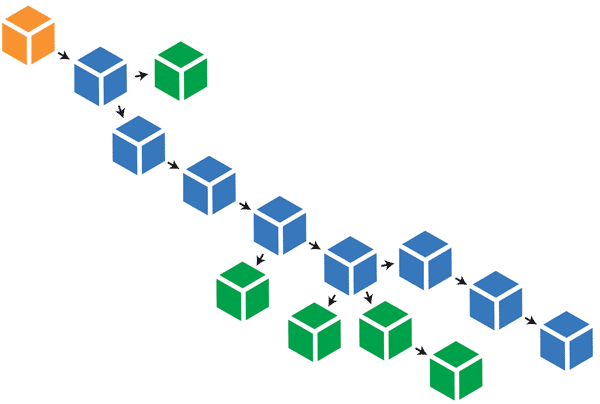
\includegraphics[width=11cm, height=8cm]{blockchain2}
\end{frame}

\begin{frame}
\frametitle{Blockchain}
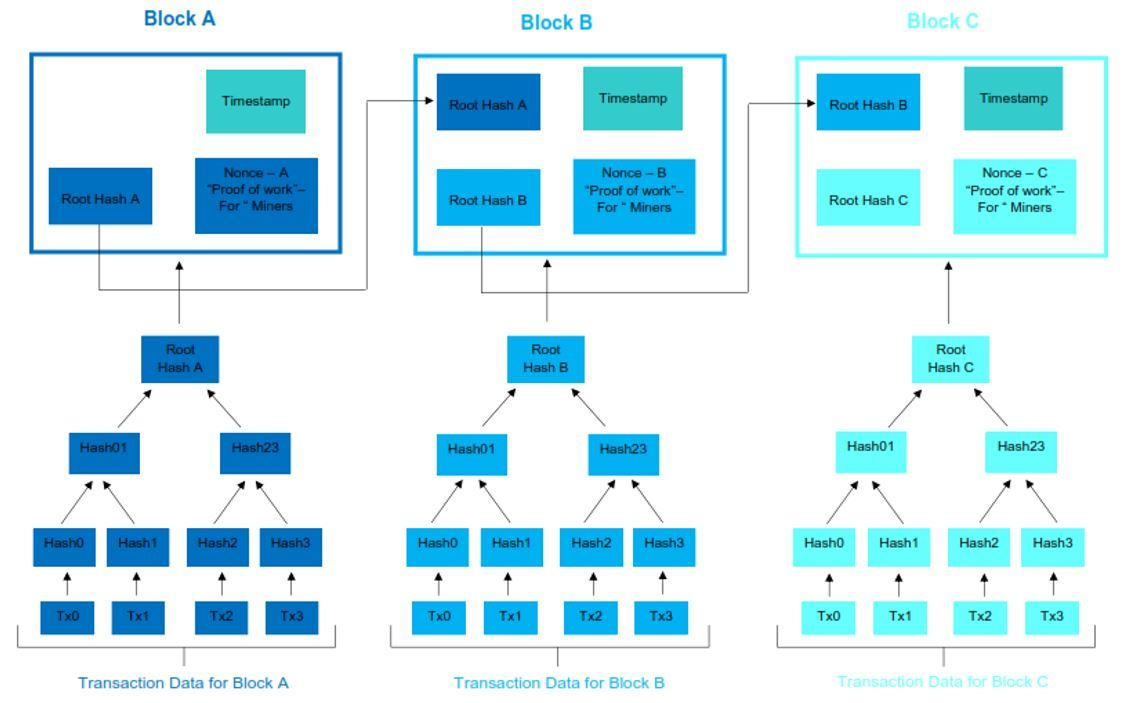
\includegraphics[width=11cm, height=8cm]{blockchain3}
\end{frame}
 
 \begin{frame}{Agda}
 \begin{itemize}
     \item Linguagem funcional e com sistema de tipos expressivo, capaz de representar especificações.
     \item Capaz de especificar e programar em um único lugar. Processo de verificação acontece no compilador.
 \end{itemize}
 \end{frame}
 
 \begin{frame}{Agda - II}
 \begin{itemize}
     \item Linguagem não possui Built-in como em Python. Tipos como inteiros, ponto flutuantes, strings, vetores deve, ser definidos pelo próprio usuário.
     \item Tipos em Agda são uma generalização de tipos de dados algébricos encontrados em Haskell e ML.
 \end{itemize}
 \end{frame}
 
 \begin{frame}{Agda --- III}
\begin{itemize}
	\item Definindo os números naturais com axiomas de peano
           \ExecuteMetaData[latex/Code.tex]{nat}
 \end{itemize}
\end{frame}

       \begin{frame}{Agda --- IV}
         \begin{itemize}
           \item Adição em Agda:
         \end{itemize}
         \ExecuteMetaData[latex/Code.tex]{plus}
\end{frame}

       \begin{frame}{Agda - V}
         \begin{itemize}
           \item Dizemos que um certo tipo é dependente se este depende de um valor.
           \item Exemplo --- Listas indexadas por seu tamanho:
         \end{itemize}
         \ExecuteMetaData[latex/Code.tex]{vector}
\end{frame}

       \begin{frame}{Agda - VI}
	\begin{adjustwidth}{-3.5em}{-2em} \fontsize{8}{11}
         \ExecuteMetaData[latex/Code.tex]{blockchain}
	\end{adjustwidth}
\end{frame}
 
 \begin{frame}
\frametitle{Objetivos}
\begin{itemize}
    \item Programar uma criptomoeda (parecida com o Bitcoin) em Agda. Uma linguagem com tipos dependentes.
    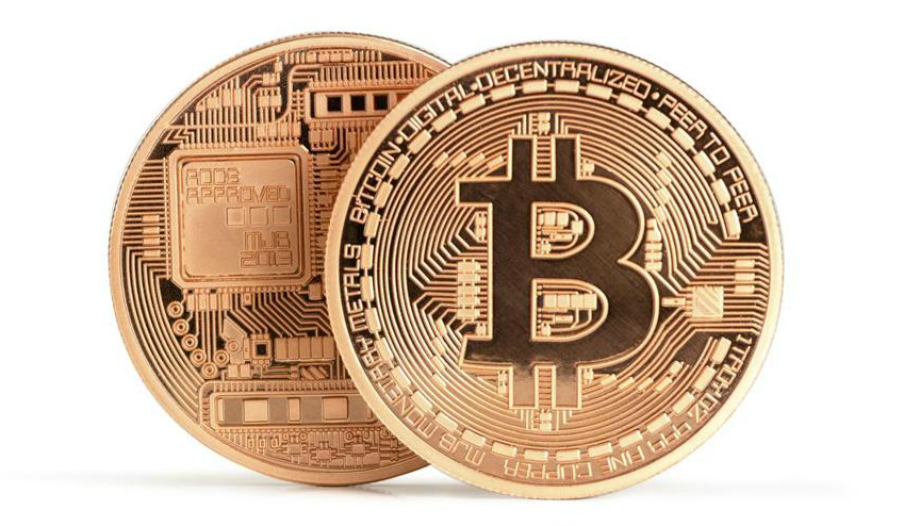
\includegraphics[width=8cm, height=5cm]{TwoBitcoins}
\end{itemize}
\end{frame}

 \begin{frame}
\frametitle{Justificativa}
\begin{itemize}
    \item Programar um protocólo de criptomoedas livre de BUGs
    \item Com Agda, além da programação da criptomoeda, temos a sua especificação de como ela deveria se comportar
\end{itemize}
\end{frame}

  \begin{frame}{O que já foi feito}
    \begin{itemize}
        \item Programada cripto-moeda em python
        \item Programada parte da blockchain em Agda
        \item Pelo paper, já foi feito parte de transações. UTXO (Unspent transaction output)
    \end{itemize}
  \end{frame}
  
  \begin{frame}{Próximos passos}
    \begin{itemize}
        \item Juntar a parte da blockchain com transações
        \item Se necessário, provar alguns teoremas relacionados ao bitcoin
    \end{itemize}
  \end{frame}
  
  \begin{frame}{Teoremas}
    \begin{itemize}
        \item Se uma transação tem algum output e ele não foi usada em nenhuma outra transação. Então ela deve estar na lista de outputs transactions não usados
        \item Se uma transação tem algum output que foi gasto. Ele não pode ser usado novamente.
        \item Provar que transações e mensagens ids são únicos
    \end{itemize}
  \end{frame}
  
  \begin{frame}{O que não será feito}
    \begin{itemize}
      \item Modelo de cripto-moeda em que é possível algum tipo de fork. No bitcoin, é possível que exista algum tipo de fork temporário
      \item Pool de transações. Sua utilidade é apenas para guardar as transações que ainda não foram adicionadas na blockchain. 
      Isso pode ser feito fora do protocolo principal
      \item Otimização e protocolos RPC. O objetivo do projeto é definir as propriedades da cripto-moeda, não como ela será implementada e usada
    \end{itemize}
  \end{frame}

 \begin{frame}{Livros}
    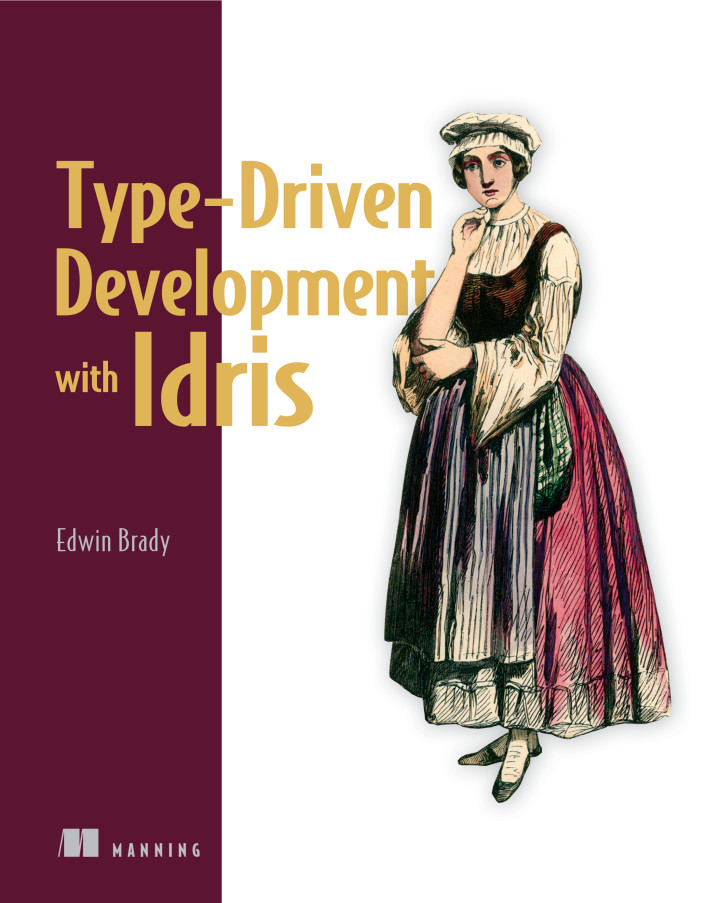
\includegraphics[width=4cm, height=6cm]{TDD}
    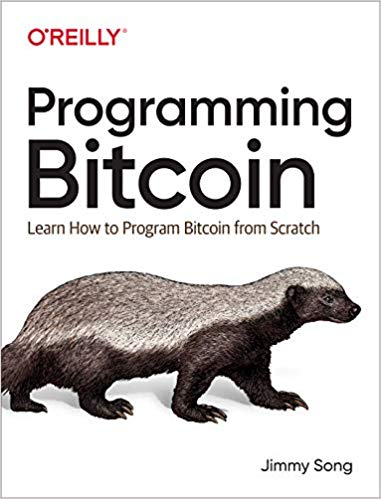
\includegraphics[width=4cm, height=6cm]{ProgrammingBitcoin}
 \end{frame}
  
\end{document}

